%******************************************************************************%
%                                                                              %
%                  html_css.en.tex                                             %
%                  Created on : Tue Mar 10 13:27:28 2015                       %
%                  Made by : Max Aghayev <maghayev@student.42.us.org>          %
%                                                                              %
%******************************************************************************%

\documentclass{42-en}


%******************************************************************************%
%                                                                              %
%                                    Header                                    %
%                                                                              %
%******************************************************************************%
\begin{document}



                           \title{Intro to Web}
                          \subtitle{Basics of HTML and CSS}
                       \member{Maksud Aghayev aka Shadow}{maghayev@student.42.us.org}
                        \member{42 Staff}{pedago@42.fr}

\summary {
  Introduction to Web World.
}

\maketitle

\tableofcontents


%******************************************************************************%
%                                                                              %
%                                  Foreword                                    %
%                                                                              %
%******************************************************************************%
\chapter{Foreword}

    We live in a time when websites have become part of our everyday lives, replacing newspapers and books, and offering humans a whole new range of opportunities to express themselves. You probably visit at least your favorite websites every day, whether it's for shopping, sending messages, playing games, checking the news or looking at pictures of your friends. Since the 1990s we have been using webistes to have fun, make a living, and talk to previously unknown people.\\

    \href{https://www.youtube.com/watch?v=aVIy54CtWXM}{YouTube Evolution 2005-2016}\\

    \href{https://www.youtube.com/watch?v=3ZD4l94IxrU}{Evolution of Facebook 2004-2016}\\

    \href{https://www.reddit.com/r/forgottenwebsites/}{r/forgottenwebsites}\\

    \href{https://archive.org/web/}{Internet Archive Wayback Machine}\\

    Have you ever wondered how to build your own piece of online real estate?

    How hard could it be?\\

    I invite you to take that journey with me.\\

    \newpage

%******************************************************************************%
%                                                                              %
%                             General instructions                             %
%                                                                              %
%******************************************************************************%
\chapter{General instructions}

    You must use HTML5 and CSS only!\\

    There are 2 \texttt{Mandatory Parts}.\\ 

    \texttt{Mandatory Parts}.
    
    Your folders must be arranged as follows:
    \begin{itemize}\itemsep1pt
        \item For mandatory part 1, create a folder named \texttt{part1} in root of the repository. This folder has to have 1 .html file with your page code.
        \item For mandatory part 2, create a folder named \texttt{part2} in root of the repository. This folder has to have 2 .html files for each part of the section.
        \item Root folder must also contain the folders: \texttt{css}, \texttt{assets}.\\
    \end{itemize}
    
    \texttt{CSS} folder can contain from 0 to * .css files.

    \texttt{Assets} folder will contain subfolders:
    \begin{itemize}\itemsep1pt
        \item \texttt{icons}. Here you can place any icons or images you would like to use.
        \item \texttt{background}\\. Here you can store background image of your choice.
    \end{itemize}

%******************************************************************************%
%                                                                              %
%                             Mandatory part                                   %
%                                                                              %
%******************************************************************************%
\chapter{Mandatory part}

    \section{Foundation and Style}
        In this section we will start by laying foundation of your web page.\\

        General instructions for this section are:
        \begin{itemize}\itemsep1pt
            \item You have to create a \texttt{grid} like page.
            \item You can style it however you like, the mandatory part is the correct structure of your page. E.g. having navigation bar, proper setting of \texttt{padding} and \texttt{margin}.
            \item Each grid block should not exceed 100x100 square.
            \item Grid blocks should be placed in logical order, 
            \item Each grid item should have a tooltip when hovered, or should have a small text that will have a name of the item.
            \item As an idea for development you can build a grid where each block will link to real websites, or to specific images that you liked on the internet. Your imagination is a limit (and school norms :))\\
        \end{itemize}
        \hint{
            Great websites have one common thing, they all have \texttt{favicon} ;)
        }
        \hint{
            Think of how you plan to style your page. There are multiple ways to create styles. You can have them \texttt{inline} or as external file. Which way to use is totally up to you. Employ \href{https://www.w3schools.com/css/css_howto.asp}{Google} to let you know what are the best practises.
        }
        \begin{figure}[H]
            \begin{center}
                \includegraphics[width=15cm]{examplep1.png}
            \end{center}
        \end{figure}
        
        \newpage
        
        
        \section{Forms and Inputs}
        In this section we will two forms and learn how input elements work. Also, as usual you have to style your form to the minimal pleasant appearance. Don't leave it in some default standard way. Imaginatiooonnn...\\

        General instructions for this section are:
        \subsection{Form for block creation}
            Create a form that will adhere to the following guidelines:
            \begin{itemize}\itemsep3pt
                \item Form should be of method POST and action should be linked to nowhere.
                \item Form should have 5 \texttt{input fields}:
                \begin{itemize}
                    \item Input field which will hold string. Maximum characters in the field should be limited to 20.
                    \item Input field which will hold string. Maximum characters in the field should be limited to 50.
                    \item Input field which will hold URL. No cap on maximum length.
                    \item Input field for file selection.
                    \item Input field for submitting the form.
                \end{itemize}
            \end{itemize}
            \begin{figure}[H]
                \begin{center}
                    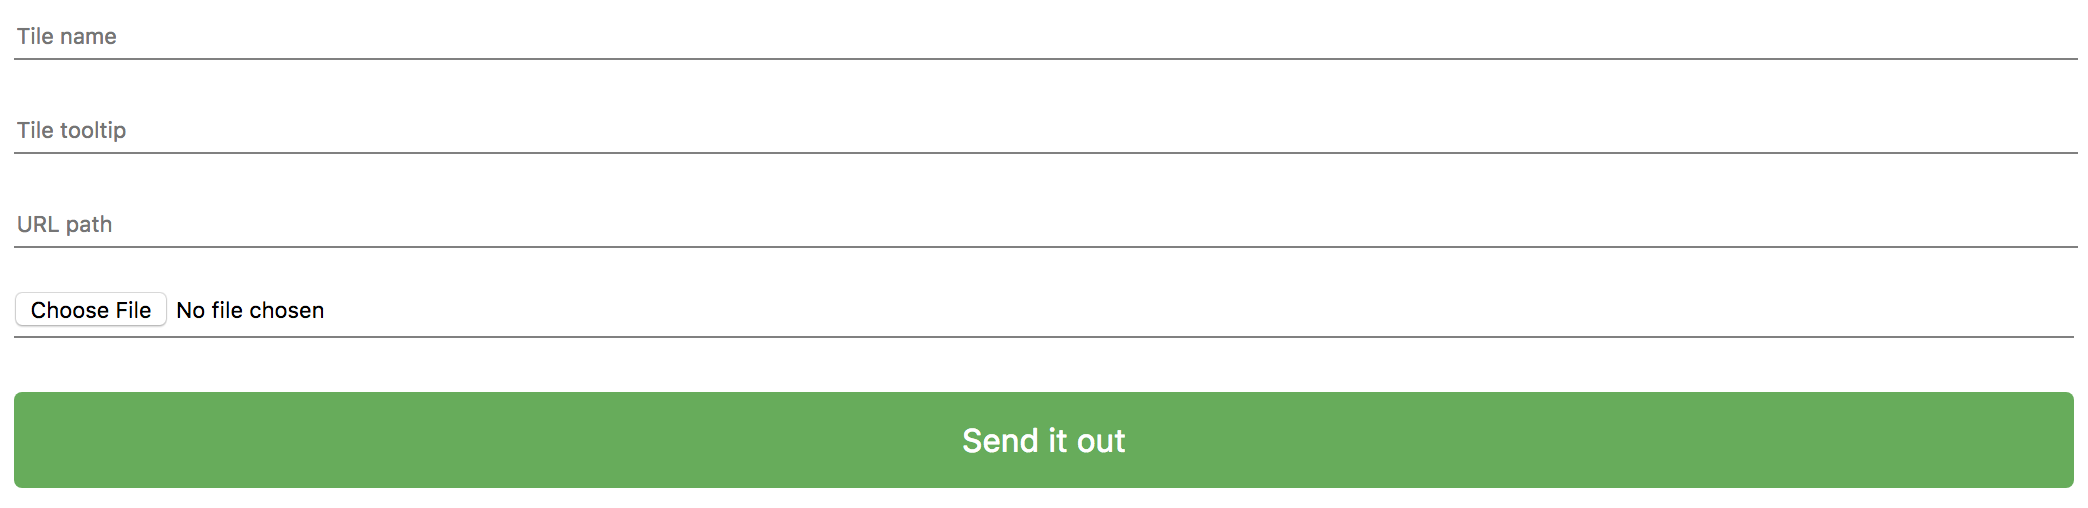
\includegraphics[width=15cm]{form1p2.png}
                \end{center}
            \end{figure}
        \subsection{Form for accepting user login and password}
        Create a form that will adhere to the following guidelines:
        \begin{itemize}\itemsep3pt
            \item Form should be of method POST and action should be linked to nowhere.
            \item Form should have 3 \texttt{input fields}:
            \begin{itemize}
                \item Input field which will hold email. No cap on maximum length.
                \item Input field which will hold password. No cap on maximum length.
                \item Input field for submitting the form.
            \end{itemize}
        \end{itemize}
        \begin{figure}[H]
            \begin{center}
                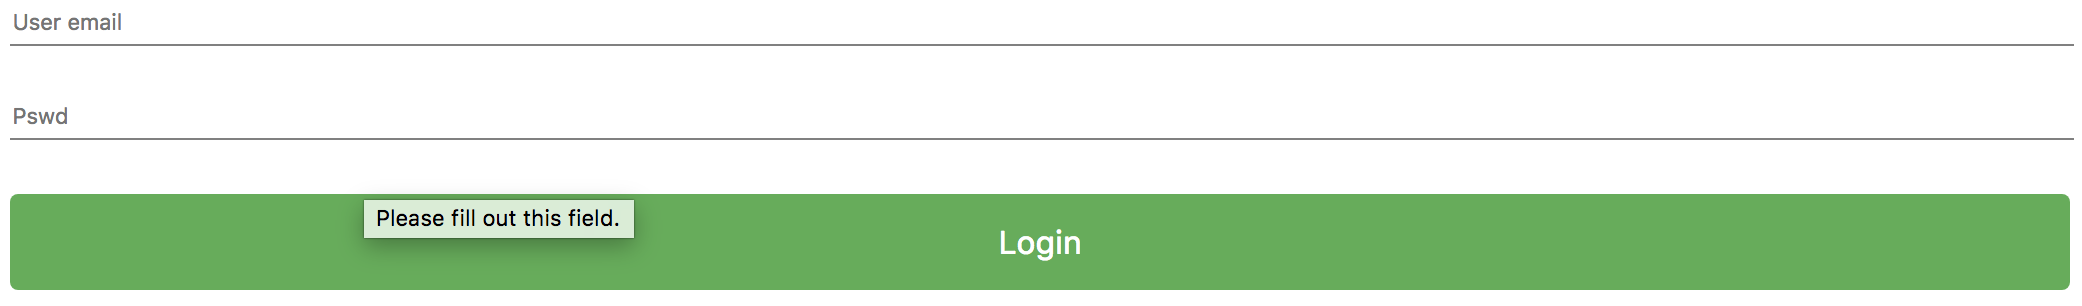
\includegraphics[width=15cm]{form2p2.png}
            \end{center}
        \end{figure}
    \hint {
      Take close look at \texttt{required} parameter of input field.
    }
    \hint{
      Think about forms the same way you would write information about someone. E.g.
      \begin{itemize}
          \item Name ...
          \item Age ....
          \item Image ..
          \item etc...
      \end{itemize}
    }


%******************************************************************************%
%                                                                              %
%                           Turn-in and peer-evaluation                        %
%                                                                              %
%******************************************************************************%
\chapter{Turn-in and peer-evaluation}

    Turn your work in using your \texttt{GiT} repository, as
    usual. Only work present on your repository will be graded in defense.

    The next project in this series will build on the scaffolding here and use Javascript to make functional forms.


%******************************************************************************%
\end{document}
